% Created 2016-11-16 Wed 11:23
\documentclass[t,10pt]{beamer}
\usepackage[utf8]{inputenc}
\usepackage[T1]{fontenc}
\usepackage{fixltx2e}
\usepackage{graphicx}
\usepackage{grffile}
\usepackage{longtable}
\usepackage{wrapfig}
\usepackage{rotating}
\usepackage[normalem]{ulem}
\usepackage{amsmath}
\usepackage{textcomp}
\usepackage{amssymb}
\usepackage{capt-of}
\usepackage{hyperref}
\mode<beamer>{\usetheme{Madrid}}
\hypersetup{colorlinks=true, linkcolor=blue}
\AtBeginSection[]{\begin{frame}<beamer>\frametitle{Topic}\tableofcontents[currentsection]\end{frame}}
\RequirePackage{fancyvrb}
\DefineVerbatimEnvironment{verbatim}{Verbatim}{fontsize=\huge}
\RequirePackage{fancyvrb}
\DefineVerbatimEnvironment{verbatim}{Verbatim}{fontsize=\scriptsize}
\RequirePackage{fancyvrb}
\DefineVerbatimEnvironment{verbatim}{Verbatim}{fontsize=\scriptsize}
\usetheme{Madrid}
\author{Stephen A. Sefick}
\date{2016-11-14}
\title{Advanced Graphics in R}

\hypersetup{
 pdfauthor={Stephen A. Sefick},
 pdftitle={Advanced Graphics in R},
 pdfkeywords={},
 pdfsubject={},
 pdfcreator={Emacs 24.3.1 (Org mode 8.3.6)}, 
 pdflang={English}}
\begin{document}

\maketitle
\begin{frame}{Outline}
\tableofcontents
\end{frame}



\section{Introduction}
\label{sec:orgheadline9}

\begin{frame}[label={sec:orgheadline1}]{Brief History: ggplot2}
\begin{itemize}
\item Data visualization system created by Hadley Wickham
\end{itemize}
\end{frame}

\begin{frame}[label={sec:orgheadline2}]{Brief History: ggplot2}
\begin{itemize}
\item Data visualization system created by Hadley Wickham
\item written in R
\end{itemize}
\end{frame}

\begin{frame}[label={sec:orgheadline3}]{Brief History: ggplot2}
\begin{itemize}
\item Data visualization system created by Hadley Wickham
\item written in R
\item Can replace base R graphics
\end{itemize}
\end{frame}

\begin{frame}[fragile,label={sec:orgheadline4}]{Brief History: ggplot2}
 \begin{itemize}
\item Data visualization system created by Hadley Wickham
\item written in R
\item Can replace base R graphics
\item Implementation of Wilkinson's Gramar of Graphics
\end{itemize}

\begin{exampleblock}{Build graphics in code blocks}
\begin{verbatim}
p <- qplot(x, y, data=df, geom="none")

p <- p+geom_boxplot()

p <- p+facet_wrap(~factor)
\end{verbatim}
\end{exampleblock}
\end{frame}

\begin{frame}[label={sec:orgheadline5}]{Motivation for using ggplot2}
\begin{itemize}
\item Very powerful and flexible
\end{itemize}
\end{frame}

\begin{frame}[label={sec:orgheadline6}]{Motivation for using ggplot2}
\begin{itemize}
\item Very powerful and flexible
\item Complete your analysis in R, and then make graphics - \alert{Reproducible Research}
\end{itemize}
\end{frame}


\begin{frame}[label={sec:orgheadline7}]{Motivation for using ggplot2}
\begin{itemize}
\item Very powerful and flexible
\item Complete your analysis in R, and then make graphics - \alert{Reproducible Research}
\item Nice output abilities to export as svg for postprocessing with Inkscape
\end{itemize}
\end{frame}

\begin{frame}[label={sec:orgheadline8}]{Motivation for using ggplot2}
\begin{itemize}
\item Very powerful and flexible
\item Complete your analysis in R, and then make graphics - \alert{Reproducible Research}
\item Nice output abilities to export as svg for postprocessing with Inkscape
\item Publication Quality Graphics
\end{itemize}
\end{frame}


\section{ggplot2 code}
\label{sec:orgheadline19}
\begin{frame}[fragile,label={sec:orgheadline10}]{qplot}
 \begin{verbatim}
qplot(x, y, data=df)
\end{verbatim}
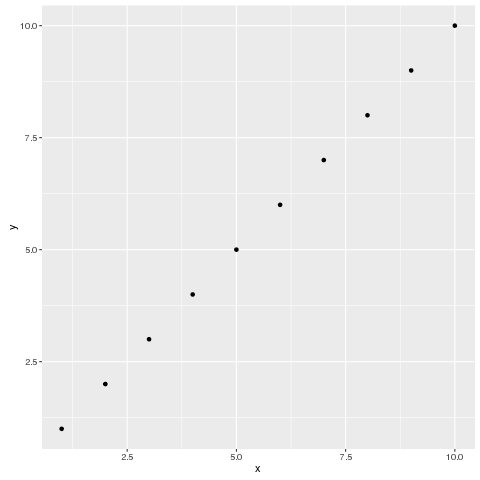
\includegraphics[width=7cm,height=7cm]{./plot.png}
\end{frame}

\begin{frame}[label={sec:orgheadline11}]{Color and shape: qplot(x, y,data=df, size=I(3)) +publication()}
\begin{columns}
\begin{column}{0.5\columnwidth}
\begin{block}{col=factor}
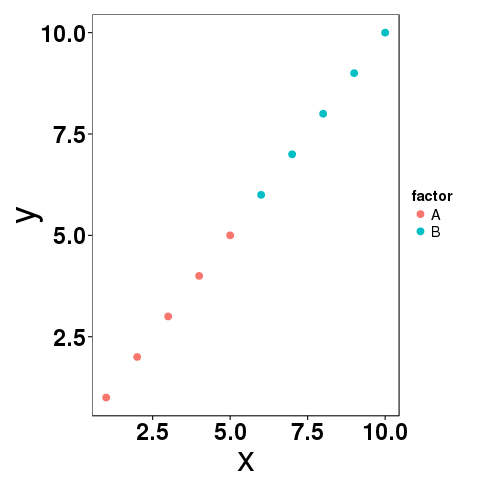
\includegraphics[width=6cm,height=6cm]{./plot_col.png}
\end{block}
\end{column}

\begin{column}{0.5\columnwidth}
\begin{block}{shape=factor}
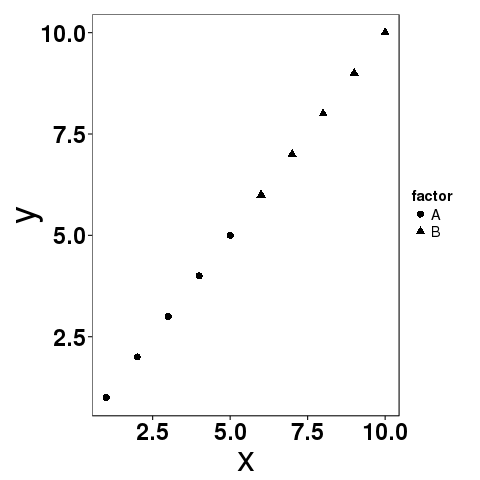
\includegraphics[width=6cm,height=6cm]{./plot_shape.png}
\end{block}
\end{column}
\end{columns}
\end{frame}

\begin{frame}[label={sec:orgheadline12}]{geoms}
\begin{itemize}
\item These are the possible "kinds" of plots you can make
\end{itemize}
selected geoms:
\begin{itemize}
\item point
\item line
\item boxplot
\item histogram
\end{itemize}
\end{frame}

\begin{frame}[label={sec:orgheadline13}]{geoms: point and line qplot(x, y, data=a, size=I(3)) +publication()}
\begin{columns}
\begin{column}{0.5\columnwidth}
\begin{block}{geom="point"}
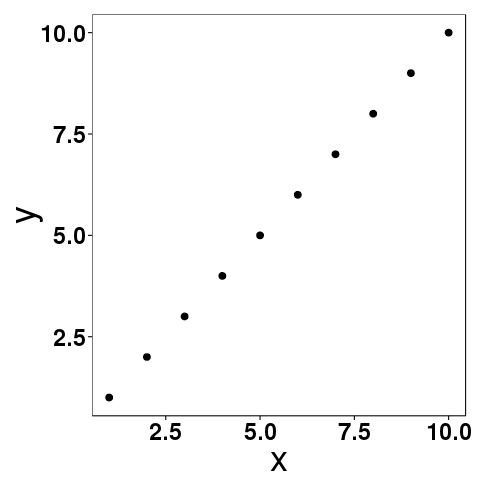
\includegraphics[width=.9\linewidth]{./point.png}
\end{block}
\end{column}

\begin{column}{0.5\columnwidth}
\begin{block}{geom="line"}
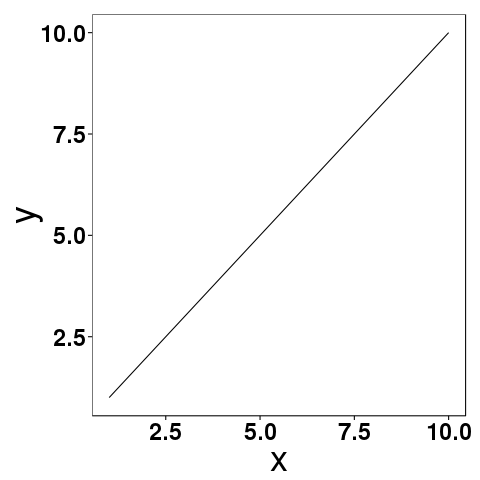
\includegraphics[width=.9\linewidth]{./line.png}
\end{block}
\end{column}
\end{columns}
\end{frame}


\begin{frame}[label={sec:orgheadline14}]{geoms: boxplot and histogram}
\begin{columns}
\begin{column}{0.5\columnwidth}
\begin{block}{qplot(factor, y, data=a, geom="boxplot")+publication()}
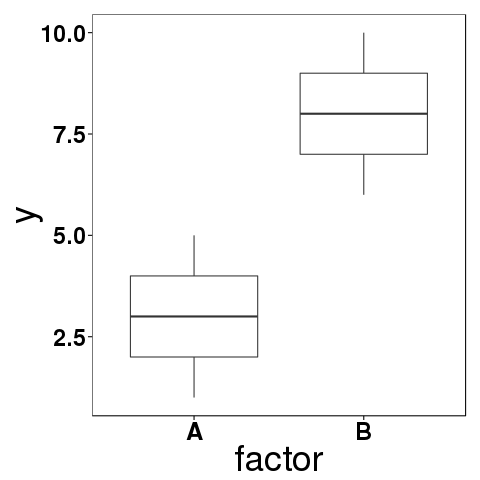
\includegraphics[width=.9\linewidth]{./boxplot.png}
\end{block}
\end{column}

\begin{column}{0.5\columnwidth}
\begin{block}{qplot(rnorm(100), geom="histogram", bins=10)+publication()}
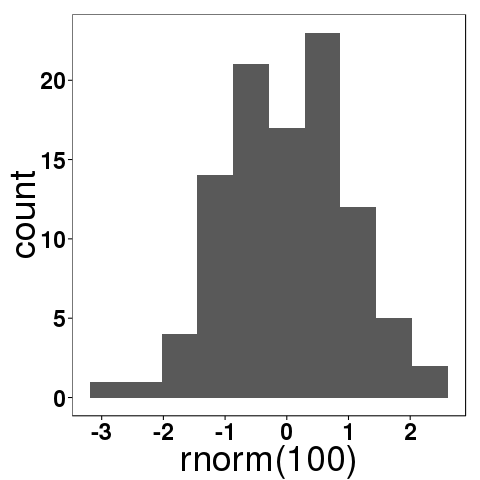
\includegraphics[width=.9\linewidth]{./histogram.png}
\end{block}
\end{column}
\end{columns}
\end{frame}


\begin{frame}[label={sec:orgheadline15}]{Base R versus ggplot2}
\begin{columns}
\begin{column}{0.5\columnwidth}
\begin{block}{Base R}
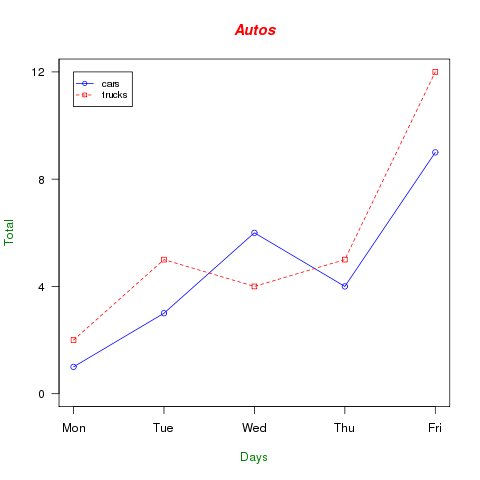
\includegraphics[width=.9\linewidth]{./Base.png}
\end{block}
\end{column}

\begin{column}{0.5\columnwidth}
\begin{block}{ggplot2}
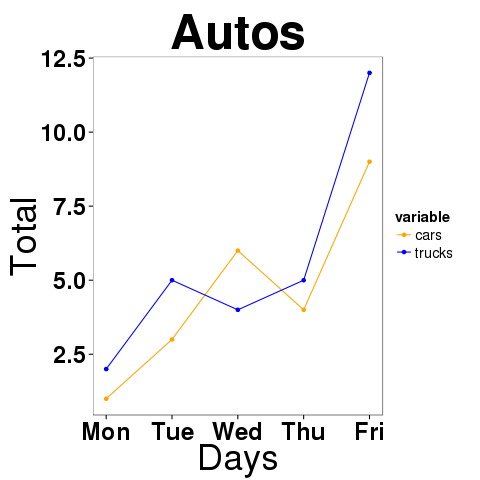
\includegraphics[width=.9\linewidth]{./Ahh_Better_ggplot2_example.png}   
\end{block}
\end{column}
\end{columns}
\end{frame}


\begin{frame}[fragile,label={sec:orgheadline16}]{Base R graphics code}
 \begin{verbatim}
#data
cars <- c(1, 3, 6, 4, 9)
trucks <- c(2, 5, 4, 5, 12)
g_range <- range(0, cars, trucks)

#plot
plot(cars, type="o", col="blue", ylim=g_range, 
   axes=FALSE, ann=FALSE)
axis(1, at=1:5, lab=c("Mon","Tue","Wed","Thu","Fri"))
axis(2, las=1, at=4*0:g_range[2])
box()
lines(trucks, type="o", pch=22, lty=2, col="red")
title(main="Autos", col.main="red", font.main=4)
title(xlab="Days", col.lab=rgb(0,0.5,0))
title(ylab="Total", col.lab=rgb(0,0.5,0))
legend(1, g_range[2], c("cars","trucks"), cex=0.8, 
   col=c("blue","red"), pch=21:22, lty=1:2);
\end{verbatim}
\end{frame}



\begin{frame}[fragile,label={sec:orgheadline17}]{ggplot graphics code}
 \begin{verbatim}
#data
library(ggplot2)
library(reshape2)
ct <- data.frame(cars = c(1, 3, 6, 4, 9), trucks = c(2, 5, 4, 5, 12), day=c(1:5))
ct.melt <- melt(ct, id.var="day")

#ggplot2
p <- qplot(day, value, data=ct.melt, col=variable)
p <- p+geom_line()
p <- p+scale_x_continuous(labels=c("Mon", "Tue", "Wed", "Thu", "Fri"))
p <- p+xlab("Days")
p <- p+ylab("Total")
p <- p+ggtitle("Autos")
p
\end{verbatim}
\end{frame}


\begin{frame}[label={sec:orgheadline18}]{Faceting: p+facet\(_{\text{wrap}}\)(\textasciitilde{}variable)}
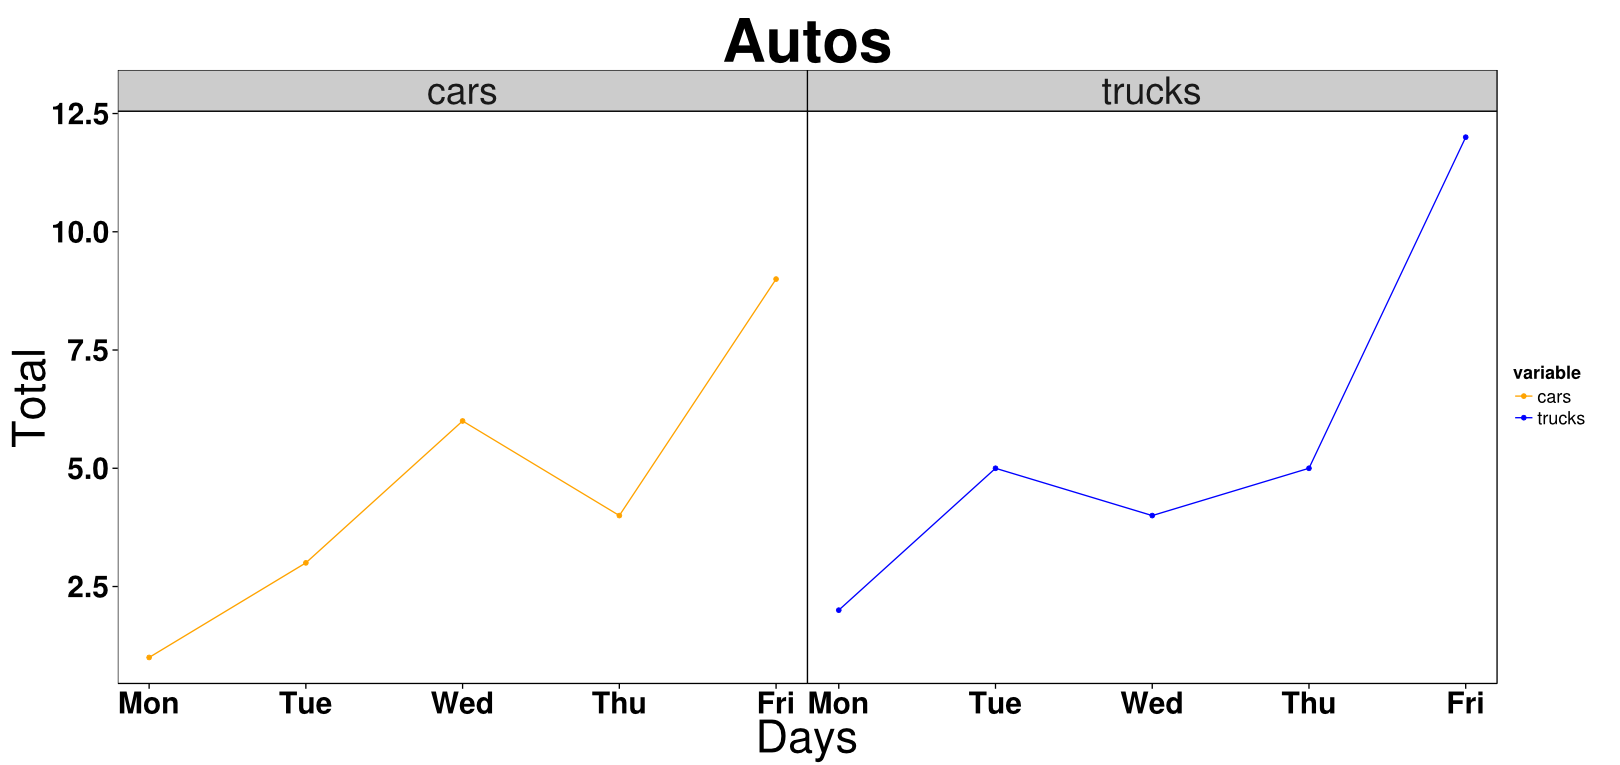
\includegraphics[width=.9\linewidth]{./faceted_plot.png}
\end{frame}

\section{Publication Quality Graphics (Examples)}
\label{sec:orgheadline22}

\begin{frame}[label={sec:orgheadline20}]{Publication Quality Graphics: Partial Least Squares}
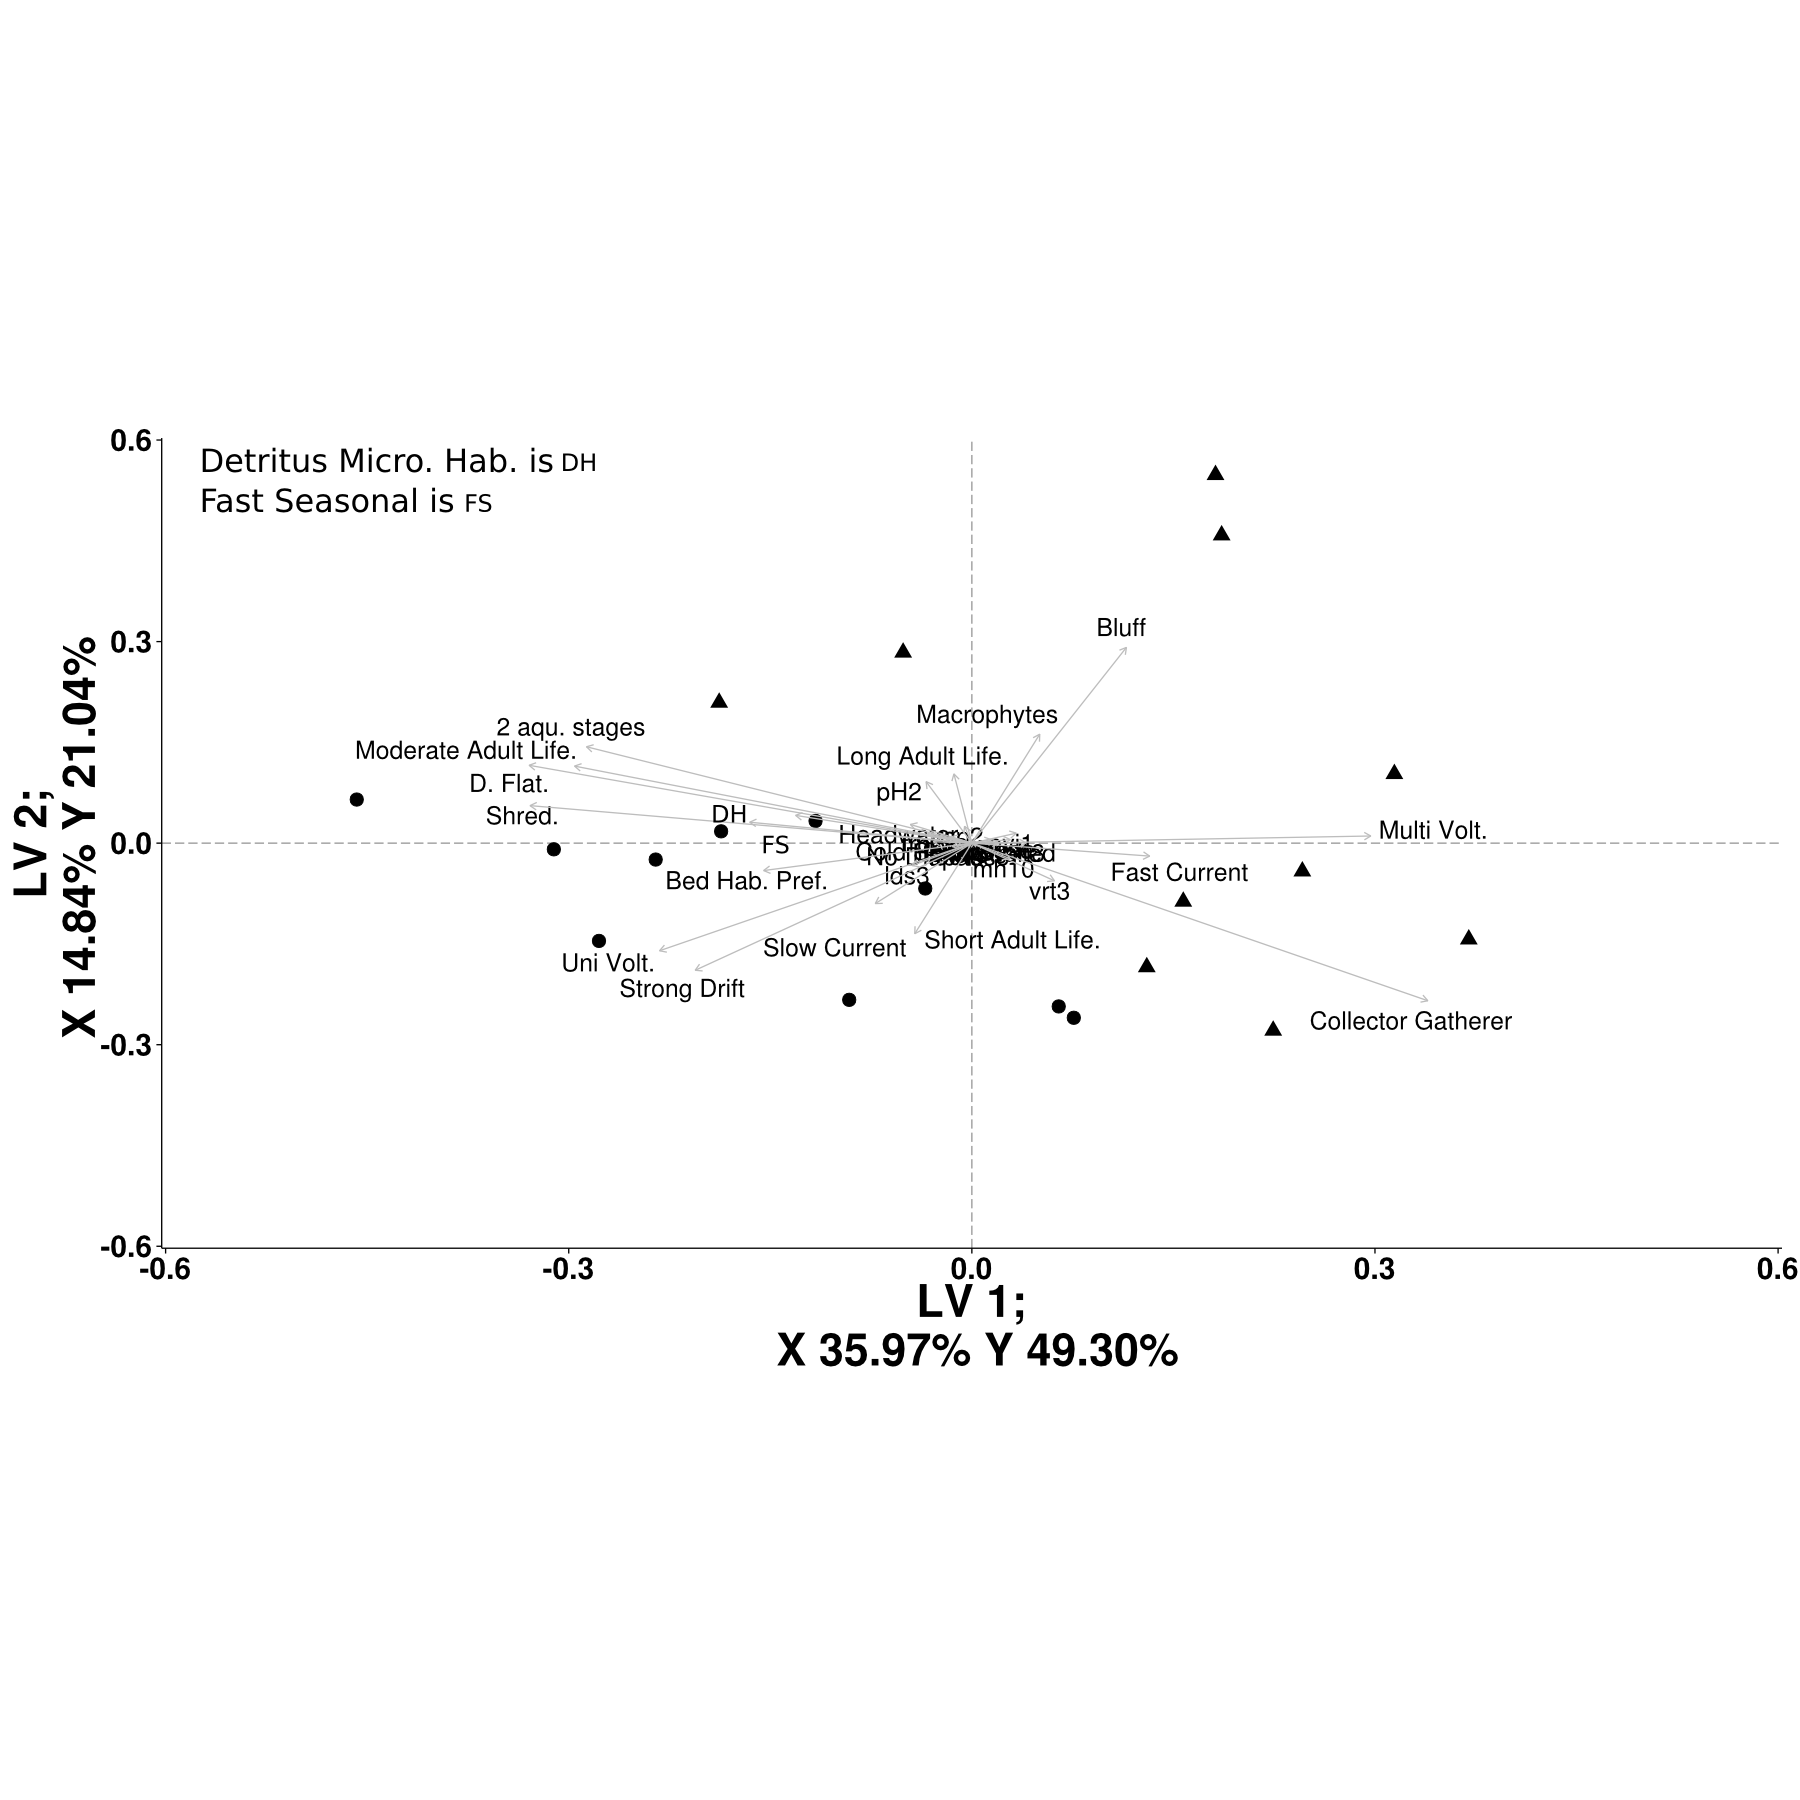
\includegraphics[width=10cm,height=10cm]{./bug.pls.out.png}
\end{frame}

\begin{frame}[label={sec:orgheadline21}]{Publication Quality Graphics: 6 panel figure}
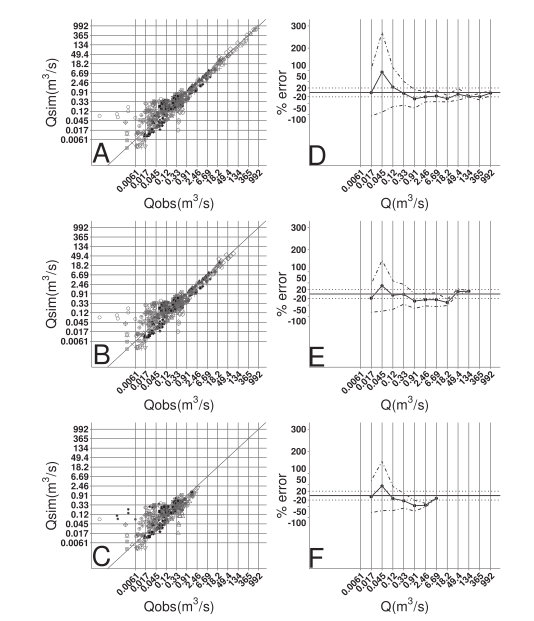
\includegraphics[width=8cm,height=8cm]{./hhydrology.png}
\end{frame}


\section{Exercises}
\label{sec:orgheadline24}
\begin{frame}[label={sec:orgheadline23}]{Let's get started}
\begin{enumerate}
\item General introduction to ggplot2

\item Velocity data from an experiment I ran in Sandy Creek

\item \alert{Questions?}
\end{enumerate}
\end{frame}
\end{document}
